\documentclass[12pt]{extarticle}
\usepackage{array}
\usepackage{booktabs} % array, booktabs to enhance tables
\usepackage{spreadtab} % to calculate into the table
\usepackage[T1]{fontenc} % addings to font
\usepackage[Russian]{babel}
\usepackage{numprint} % to create beautiful numbers
\usepackage[margin=3cm]{geometry}
\usepackage{float} % to set position of table or figure on a page ([H])
\usepackage{xfp}
\usepackage{amsmath}
\usepackage{graphicx}

\begin{document}
\author{Осипов Александр Б06-604}
\title{Лабораторная работа 1.2.3. Опеределение моментов инерции твёрдых тел с помощью трифилярного подвеса}
\maketitle
\section{Цель}

Измерение момента инерции ряда тел и сравнение результатов с теоретическими расчётами.

\section{Оборудование}

Трифилярный подвес, секундомер, счётчик числа колебаний, набор тел.

\section{Ход работы}
\subsection{Измерение параметров установки:}

\vspace{5mm}

$l = 216 \text{ cm}$

$R = 115.5 \text{ mm}$

$\sigma_r = 0.3 \text{ mm}$

$r = 30.2 \text{ mm}$

$\sigma_R = 0.5 \text{ mm}$ 

$z = (l^2 - R^2)^{0.5} =  2.16 \text{ m}$

\newpage

\subsection{Расчет константы k установки и её ошибки:}
$$\displaystyle \frac{\partial}{\partial r} k{\left(r,R,l \right)} = \frac{R g}{4 \pi^{2} \left(- R^{2} + l^{2}\right)}$$
\vspace{3mm}

$$\displaystyle \frac{\partial}{\partial R} k{\left(r,R,l \right)} = \frac{R^{2} g r}{2 \pi^{2} \left(- R^{2} + l^{2}\right)^{2}} + \frac{g r}{4 \pi^{2} \left(- R^{2} + l^{2}\right)}$$

\vspace{3mm}

$$\displaystyle \frac{\partial}{\partial l} k{\left(r,R,l \right)} = - \frac{R g l r}{2 \pi^{2} \left(- R^{2} + l^{2}\right)^{2}}$$

\vspace{3mm}

$$\displaystyle \sigma_{k} = \sqrt{\left(\Delta{R} \left(\frac{R^{2} g r}{4 \pi^{2} \left(- R^{2} + l^{2}\right)^{\frac{3}{2}}} + \frac{g r}{4 \pi^{2} \sqrt{- R^{2} + l^{2}}}\right)\right)^{2} + \left(\frac{R \Delta{r} g}{4 \pi^{2} \sqrt{- R^{2} + l^{2}}}\right)^{2} + \left(- \frac{R \Delta{l} g l r}{4 \pi^{2} \left(- R^{2} + l^{2}\right)^{\frac{3}{2}}}\right)^{2}}$$

\vspace{3mm}

$k = (4 \pm 0.04) \cdot 10^{-4}$

\subsection{Измерение момента инерции:}

Основная формула для расчета:

$$\displaystyle I = \frac{R T^{2} g m r}{4 \pi^{2} \left(- R^{2} + l^{2}\right)}$$

\subsubsection{Платформа:}

$m = 1026.4*10^{-3}$

$\sigma_m = 0.5*10^{-3}$

$I_{platform} = 0.01264$

\vspace{3mm}

\textbf{\large{Момент инерции пустой платформы:}}

\vspace{3mm}

$\displaystyle I = 8 \cdot 10^{-3}$
\vspace{3mm}


Расёт ошибки момента инерции пустой платформы:

$$\displaystyle \frac{\partial}{\partial k} I_{0}{\left(k,m_{0},T_{0} \right)} = T_{0}^{2} m_{0}$$

\vspace{3mm}

$$\displaystyle \frac{\partial}{\partial m_{0}} I_{0}{\left(k,m_{0},T_{0} \right)} = T_{0}^{2} k$$

\vspace{3mm}

$$\displaystyle \frac{\partial}{\partial T_{0}} I_{0}{\left(k,m_{0},T_{0} \right)} = 2 T_{0} k m_{0}$$

\vspace{3mm}

$$\displaystyle \sigma_{I_0} = \sqrt{T_{0}^{4} \sigma_{k}^{2} m_{0}^{2} + T_{0}^{4} \sigma_{m_0}^{2} k^{2} + 4 T_{0}^{2} \sigma_{T_0}^{2} k^{2} m_{0}^{2}}$$

\vspace{3mm}

$\displaystyle \sigma_{I_0} = 8.73881755020746 \cdot 10^{-5}$

\subsubsection{Тела 1(круг) и 2(брусок), проверка аддитивности моментов:}
\vspace{3mm}

\large{Тело 1}
\vspace{3mm}

\begin{tabular}{lcc}
\toprule
 & t, c & n \\
\midrule
0 & 118.96 & 30 \\
1 & 98.8& 25 \\
2 & 79.19 & 20 \\
\bottomrule
\end{tabular}

\vspace{3mm}

\large{Тело 2:}
\vspace{3mm}

\begin{tabular}{lrr}
\toprule
 & t, c & n \\
\midrule
0 & 112.540000 & 30 \\
1 & 93.550000 & 25 \\
2 & 74.990000 & 20 \\
\bottomrule
\end{tabular}

\vspace{3mm}

\large{Совместное измерение:}
\vspace{3mm}

\begin{tabular}{lrr}
\toprule
 & t, с & n \\
\midrule
0 & 107.560000 & 30 \\
1 & 89.640000 & 25 \\
2 & 72.000000 & 20 \\
\bottomrule
\end{tabular}

\vspace{3mm}

$\displaystyle I_{1} = - T_{0}^{2} k m_{0} + T_{1}^{2} k \left(m_{0} + m_{1}\right)$

\vspace{3mm}

$\displaystyle I_{2} = - T_{0}^{2} k m_{0} + T_{2}^{2} k \left(m_{0} + m_{2}\right)$

\vspace{3mm}

$\displaystyle I_{12} = - T_{0}^{2} k m_{0} + T_{12}^{2} k \left(m_{0} + m_{1} + m_{2}\right)$


Тело 1:
\vspace{3mm}

$I_1 = (0.00212 \pm 0.00003) \text{ kg} \cdot \text{m}^2$
\vspace{3mm}

Тело 2:
\vspace{3mm}

$I_2 = (0.00493 \pm 0.00006) \text{ кг} \cdot \text{ь}^2$

\vspace{3mm}

Оба тела:
\vspace{3mm}
$I_{12} = (0.00691 \pm 0.00009) \text{ кг} \cdot \text{м}^2$


\vspace{5mm}

\textbf{\large{Проверка адддитивности:}}

\vspace{3mm}

По формуле $\displaystyle \Delta I = - I_{1} + I_{12} - I_{2}$

\vspace{3mm}

Отличие теоретической суммы моментов от полученной экспериментально:

\vspace{3mm}

$\Delta_I = (-0.000139 \pm 0.000049) \text{ кг} \cdot \text{м}^2$ 

\vspace{5mm}

\textbf{\large{Сравнение с теоретическими значениями:}}

\vspace{3mm}

$\displaystyle I_{1,\mathrm{theory}} = \frac{m_{1} r_{1}^{2}}{2}$

\vspace{3mm}

$\displaystyle I_{2,\mathrm{theory}} = \frac{m_{2} \left(d_{2}^{2} + w_{2}^{2}\right)}{12}$

\vspace{3mm}

\begin{tabular}{cccc}
\toprule
Тело & Эксперимент, кг·м² & Теория, кг·м² & Отклонение, \% \\
\midrule 
диск & 4.807186 & 2.774392 & 73.269894 \\
брусок & 0.004928 & 0.004735 & 4.084469 \\
\bottomrule
\end{tabular}

\subsubsection{Момент инерции разрезанного диска}

\vspace{5mm}

\begin{tabular}{lrrr}
\toprule
 & h & t, с & n \\
\midrule
0 & 0 & 77.250000 & 25 \\
1 & 5 & 77.060000 & 25 \\
2 & 15 & 78.340000 & 25 \\
3 & 30 & 82.460000 & 25 \\
4 & 40 & 86.020000 & 25 \\
5 & 55 & 93.360000 & 25 \\
6 & 65 & 99.020000 & 25 \\
\bottomrule
\end{tabular}

\vspace{5mm}

$\displaystyle I_{d} = - T_{0}^{2} k m_{0} + T_{d}^{2} k \left(m_{0} + m_{d}\right)$

\vspace{5mm}

$\displaystyle \sigma_{I_d} = \sqrt{4 T_{0}^{2} \sigma_{T_0}^{2} k^{2} m_{0}^{2} + T_{d}^{4} \sigma_{m_d}^{2} k^{2} + 4 T_{d}^{2} \sigma_{T_d}^{2} k^{2} \left(m_{0} + m_{d}\right)^{2} + \sigma_{k}^{2} \left(- T_{0}^{2} m_{0} + T_{d}^{2} \left(m_{0} + m_{d}\right)\right)^{2} + \sigma_{m_0}^{2} \left(- T_{0}^{2} k + T_{d}^{2} k\right)^{2}}$

\vspace{3mm}

Результирующая таблица с моментом инерци:

\vspace{3mm}

\begin{tabular}{lrrrrrrr}
\toprule
 & h & t, с & n & T, c & $\sigma_T, \text{c}$ & $I, \text{кг}\cdot\text{м}^2$ & $\sigma_I, \text{кг} \cdot \text{м}^2 $\\
\midrule
0 & 0 & 77.250000 & 25 & 3.090000 & 0.000400 & 0.001750 & 0.000019 \\
1 & 5 & 77.060000 & 25 & 3.082400 & 0.000400 & 0.001702 & 0.000019 \\
2 & 15 & 78.340000 & 25 & 3.133600 & 0.000400 & 0.002028 & 0.000023 \\
3 & 30 & 82.460000 & 25 & 3.298400 & 0.000400 & 0.003116 & 0.000034 \\
4 & 40 & 86.020000 & 25 & 3.440800 & 0.000400 & 0.004101 & 0.000045 \\
5 & 55 & 93.360000 & 25 & 3.734400 & 0.000400 & 0.006263 & 0.000068 \\
6 & 65 & 99.020000 & 25 & 3.960800 & 0.000400 & 0.008051 & 0.000087 \\
\bottomrule
\end{tabular}


\vspace{5mm}

\begin{center}
  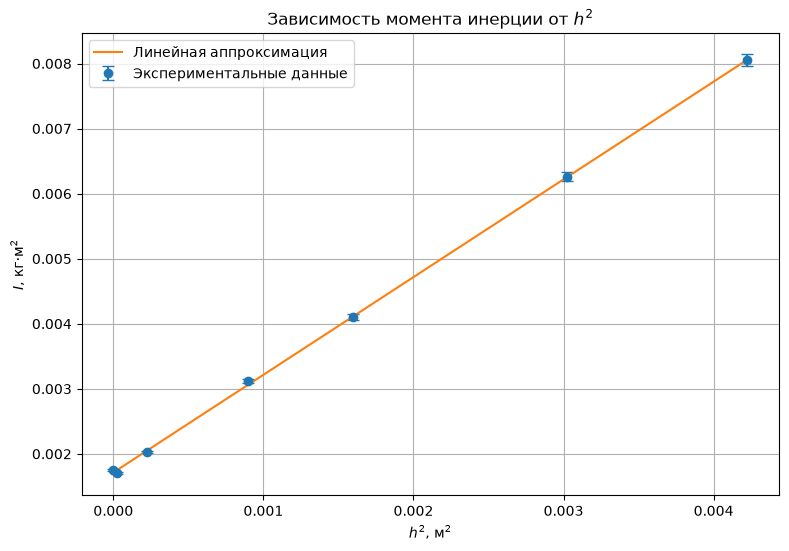
\includegraphics[scale=0.85]{../assets/1_2_3/plot.png}
\end{center}

\vspace{5mm}
Масса одной половинки: m = 0.7511 кг
\vspace{3mm}

Масса всего диска: M = 1.5021 кг

\section{Вывод:}

Были измерены момент инерции различных тел, установлена зависимость
момент инерции от квадрата расстояния между центральными частями для разрезанного диска.

\end{document}